\documentclass[a4paper,12pt,oneside]{memoir}

%matematički paketi

\usepackage[intlimits]{amsmath}     %omogućava postavljanje granica integrala u formulama
\usepackage{amsthm}         %matematički teoremi, leme i sl.
\usepackage{siunitx}        %podrška za korištenje SI sustava mjernih jedinica

%encoding fontova i jezika
\usepackage[croatian]{babel}
\usepackage[utf8x]{inputenc}        %encoding inputa
\usepackage[enc=utf8]{hrlatex}
\usepackage[T1]{fontenc}        %encoding fontova koji je prikazan u PDF-u
\usepackage{amsfonts}
\usepackage{dsfont}

\usepackage[fixlanguage]{babelbib}
\selectbiblanguage{croatian}
\OnehalfSpacing

%\usepackage[datetime2-croatian]{datetime2}

%paketi tablica, naslova, poglavlja i sl.
\usepackage[thinlines]{easytable}
\usepackage{tocloft}        %upravljanje izgledom tablice sadržaja
\usepackage{pdfpages}       %integracija eksternih PDF-ova
\usepackage{booktabs}       %koristi se za formatiranje tablica sukladno standardu za znanstvene radove i članke
\usepackage{indentfirst}     %dodaje tab za svaku prvu rečenicu odlomka
\usepackage{subcaption}     %koristi se za podnaslove slika, formi i sl.
\usepackage[font=it]{caption}
\captionsetup[table]{position=above}
\captionsetup[figure]{position=below}
\captionsetup{labelsep=period}

\usepackage[hidelinks]{hyperref}        %podrška za integraciju hyperlinkova
\urlstyle{same}

\usepackage{float}
%grafički paketi
% \usepackage{pgfcore}
% \usepgflibrary{datavisualization.formats.functions}
\usepackage{graphicx}
\usepackage{pgfmath}
\usepackage{pgfplots}
\pgfplotsset{compat=1.17}
\pgfplotsset{
    standard/.style={
        width = 7cm,
        semithick,
        tick style={major tick length=4pt,semithick,black},
        every axis plot post/.style={mark options={fill=black}},
        separate axis lines,
        axis x line*=bottom,
        axis x line shift=10pt,
        %xlabel shift=5pt,
        axis y line*=left,
        axis y line shift=10pt,
        %ylabel shift=0pt,
        xtick align = outside,
        ytick align = outside,
        xlabel near ticks,
        ylabel near ticks,
        xmin = -1, xmax = 1,
        ymin = -1, ymax = 1,
        grid
    }
}
\usepackage{tikz}
\usetikzlibrary{datavisualization}
\usetikzlibrary{datavisualization.formats.functions}
\usetikzlibrary{arrows,automata,patterns,positioning}
\usepackage{circuitikz}
\newcommand{\pgfmathparseFPU}[1]{\begingroup%
\pgfkeys{/pgf/fpu,/pgf/fpu/output format=fixed}%
\pgfmathparse{#1}%
\pgfmathsmuggle\pgfmathresult\endgroup}


%misc. paketi

\usepackage{soul} %žuti marker
\usepackage{times}

%formatiranje dokumenta
\pagestyle{myheadings}
\setulmarginsandblock{2.5cm}{2.5cm}{*}
\setlrmarginsandblock{2.5cm}{2cm}{*}
\checkandfixthelayout

\setlength{\parskip}{6pt} %razmak između odlomaka

\usepackage{titlesec}   %nadomješta LaTeX makroe za naslove, odlonke, itd.

\titleformat{\chapter}
{\normalfont\fontsize{14}{14}\bfseries}
{\thechapter}
{1em}
{}
\titlespacing{\chapter}{0pt}{*4}{*1}
\titleformat{\section}
{\normalfont\fontsize{12}{14}\bfseries}
{\thesection}
{1em}
{}
\titlespacing{\section}{0pt}{*4}{*1}
\setsecnumdepth{subsection}
\maxtocdepth{subsection}
\titleformat{\subsection}
{\normalfont\fontsize{12}{14}}
{\thesubsection}
{1em}
{}
\titlespacing{\subsection}{0pt}{*4}{*1}

\begin{document}
    \begin{figure}[H]
        %\centering
        \begin{minipage}[b] {.4\linewidth}
            \centering
            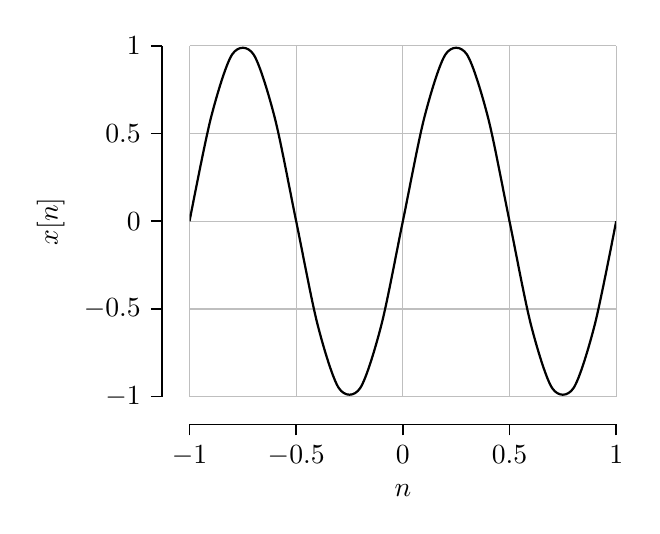
\begin{tikzpicture}
                \begin{axis}[
                    standard,
                    xlabel={$n$},
                    ylabel={$x[n]$},
                    enlarge x limits=false,
                    domain = -1:1,
                    samples = 21,                         
                ],
                    \addplot [smooth, black, thick] {sin(2*180*x)};
                \end{axis} 
            \end{tikzpicture}
            \subcaption{Continous signal}
            \label{fig:M31}
        \end{minipage}
        \qquad\qquad
        \begin{minipage}[b] {.4\linewidth}
            \centering
            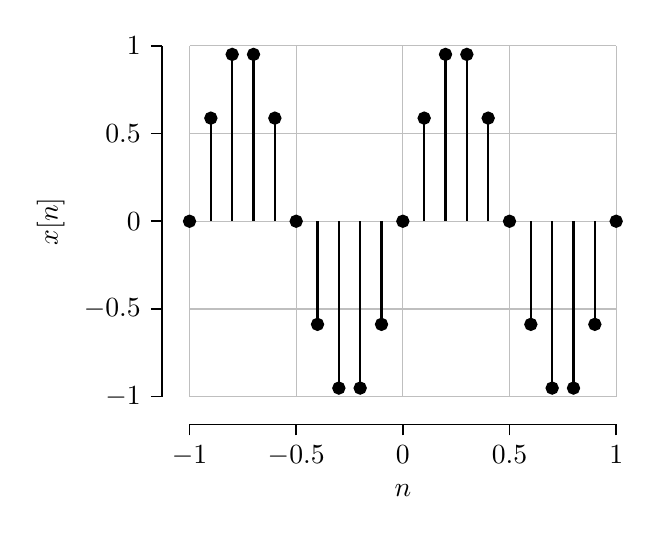
\begin{tikzpicture}
                \begin{axis}[
                    standard,
                    xlabel={$n$},
                    ylabel={$x[n]$},
                    enlarge x limits=false,
                    domain = -1:1,
                    samples = 21,                         
                ],
                    \addplot+[ycomb, black, thick] {sin(2*180*x)};
                \end{axis} 
            \end{tikzpicture}
            \subcaption{Discrete signal}      
            \label{fig:M32}
        \end{minipage}
        \caption{Main caption}
        \label{fig:M3}    
    \end{figure}
\end{document}